%---------------------------------- Large Language Models -------------------------------
\begin{frame}{Large Language Models}
\begin{columns}
      
    \begin{column}[t]{0.4\textwidth}
    \begin{block}{Summary}
    
        \begin{itemize}
            \item State-of-the-art of Natural Language Processing (NLP) problems
            \item Architecture : Transformers\cite{NIPS2017_3f5ee243} block, mixed with classical layers (MLP, Conv)
            \item 2 phases of training : pre-training and fine-tuning
        \end{itemize}
            

    \end{block}
    \end{column}
        
    \begin{column}[t]{0.6\textwidth}
    \begin{block}{Self Attention }

        \begin{figure}
            \centering
            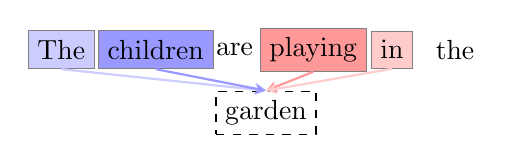
\begin{tikzpicture}[node distance=0.8cm]

    % Define block styles
    \tikzstyle{model} = [rectangle,rounded corners, minimum width=2cm, minimum height=1cm, text centered, draw=black, fill=blue!30]
    \tikzstyle{arrow} = [thick,->,>=stealth]
    
    % Define nodes
    \node (the) [fill=blue!20,rectangle,draw=black!50] {The};
    \node (children) [right of = the,fill=blue!40,rectangle,draw=black!50,xshift=0.4cm] {children};
    \node (are) [right of = children,xshift=0.2cm] {are};
    \node (playing) [right of = are,fill=red!40,rectangle,draw=black!50,xshift=0.2cm] {playing};
    \node (in) [right of = playing,fill=red!20,rectangle,draw=black!50,xshift=0.2cm] {in};
    \node (the2) [right of = in] {the};
    
    \node (garden) [below of = are, xshift=0.4cm,rectangle,dashed,draw=black] {garden};
    
    % Draw arrows
    \draw [arrow,draw=blue!20] (the.south) -- (garden.north);
    \draw [arrow,draw=blue!40] (children.south) -- (garden.north);
    \draw [arrow,draw=red!40] (playing.south) -- (garden.north);
    \draw [arrow,draw=red!20] (in.south) -- (garden.north);
    
    % Add a rectangle around the last four nodes
    \end{tikzpicture}
            \caption{Scaled dot product attention}
            \hfill
        \end{figure}
    

    \end{block}
    \end{column}
         
\end{columns}
\end{frame}


%---------------------------------- Fine Tuning Frame -------------------------------
\begin{frame}{Fine Tuning}

    \begin{block}{Parameters Efficient Fine-Tuning (PEFT)}
    Set of methods aims to reduce the computation cost of fine-tuning. Can change the structure like the 2 following, or just reduce the cost like Quantization (reduce the precision of calculus). These methods are often hyperparameter-dependent.
    \end{block}
    
    \begin{columns}  
  
        \begin{column}[t]{0.45\textwidth}
        \begin{block}{Low Rank Adaptation (LoRA)\cite{hu2021loralowrankadaptationlarge}}
                   Use of low rank matrices of the weights matrices, which will be the only ones trained, to reduce the cost of gradient computations.  
        \end{block}
        \end{column}
    
        \begin{column}[t]{0.45\textwidth}
        \begin{block}{Adapter Layer}
            Add layer inside the model, and train only these. One con is to add inference for predicting.
            
        \end{block}
        \end{column}
      
    \end{columns}

\end{frame}

%---------------------------------- Fine-tuning Workflow -------------------------------

\begin{frame}{Fine-Tuning workflow}
    
    \begin{figure}
        \centering
        \begin{tikzpicture}[node distance=1.5cm]

% Define block styles
\tikzstyle{model} = [rectangle,rounded corners, minimum width=2cm, minimum height=1cm, text centered, draw=black, fill=blue!30]
\tikzstyle{data} = [rectangle, rounded corners, minimum width=2cm, minimum height=1cm,text centered, draw=black, fill=yellow!30]
\tikzstyle{action} = [rectangle, rounded corners, minimum width=2cm, minimum height=1cm,text centered, draw=black, fill=red!30]
\tikzstyle{arrow} = [thick,->,>=stealth]

% Define nodes
\node (model1) [model,align=center] {Model\\Random init};
\node (data1) [data, below of=model1,align=center]{Pre-Training \\ Data Corpus} ;
\node (pre-train)[action, right of=model1, xshift=1.5cm,yshift=-1cm]{Pre-Training};
\node (model2) [model, right of=pre-train, xshift = 1.5cm, yshift=1cm ]{Pre-Trained Model};
\node (data2) [data, below of= model2]{In-domain data};
\node (fine-tuning)[action, right of = model2, xshift = 1.5cm,yshift=-1cm]{Fine Tuning};
\node (model3) [model, right of=fine-tuning, xshift = 1.5cm,align=center ]{Fine-Tuned \\ model};


% Draw arrows
\draw [arrow] (data1) -- (pre-train);
\draw [arrow] (model1) -- (pre-train);
\draw [arrow] (pre-train) -- (model2);
\draw [arrow] (model2) -- (fine-tuning);
\draw [arrow] (data2) -- (fine-tuning);
\draw [arrow] (fine-tuning) -- (model3);

% Add a rectangle around the last four nodes
\node[draw, thick, dashed, rounded corners, fit=(model2) (fine-tuning) (model3) (data2), inner sep=0.3cm, label=above:{Fine-Tuning Framework}] {};
\end{tikzpicture}
        \caption{Pre-training and Fine-tuning generic workflow}
    \end{figure}  
        

    
\end{frame}

%---------------------------------- LoRA -------------------------------
\begin{frame}{Low Rank Adaptation (LoRA)}
    \begin{block}{Principle}
        Merging Fine-tuning layers with pre-trained ones can be written as $W = W_0 + \Delta W$, with $W_0$ the pre-trained weights and $\Delta W$ the fine-tuned ones.         
    \end{block}

    \begin{columns}
        \begin{column}[t]{0.45\textwidth}
        \begin{figure}
            \centering
            %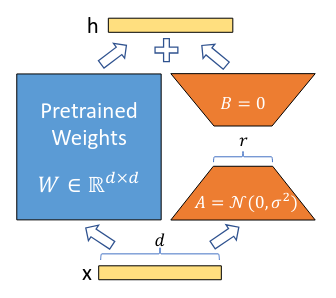
\includegraphics[width=0.5\linewidth]{imgs/lora.png}
            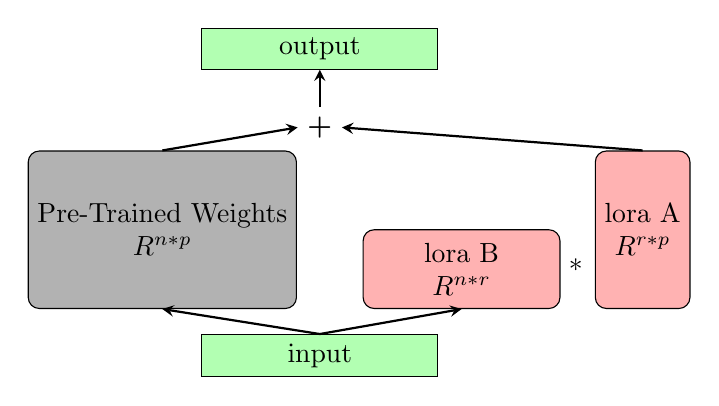
\begin{tikzpicture}[node distance=1.8cm]
    % Define block styles
    \tikzstyle{weights} = [rectangle,rounded corners, minimum width=2.5cm, minimum height=2cm, text centered, draw=black, fill=black!30]
    \tikzstyle{lora_a} = [rectangle,rounded corners, minimum width=1cm, minimum height=2cm, text centered, draw=black, fill=red!30]
    \tikzstyle{lora_b} = [rectangle,rounded corners, minimum width=2.5cm, minimum height=1cm, text centered, draw=black, fill=red!30]
    \tikzstyle{vector} = [rectangle, minimum width=3cm, minimum height=0.5cm, text centered, draw=black, fill=green!30]
    \tikzstyle{arrow} = [thick,->,>=stealth]
    
    % Define nodes
    \node (weights) [weights, align=center]{Pre-Trained Weights \\ $\mathbb{R}^{n*p}$};
    \node (lora_B) [lora_b, right of=weights,xshift=2cm,yshift=-0.5cm, align=center]{lora B\\ $\mathbb{R}^{n*r}$};
    \node (mul) [right of = lora_B,xshift=-0.35cm]{*};
    \node (lora_A) [lora_a, right of=lora_B,xshift=0.5cm,yshift=0.5cm, align=center]{lora A\\$\mathbb{R}^{r*p}$};
    \node (input) [vector,below of = weights, xshift = 2cm,yshift=+0.2cm]{input};
    \node (plus) [above of = weights, xshift = 2cm,yshift=-0.5cm]{\textbf{+}};
    \node (output) [vector,above of = plus,yshift=-0.8cm]{output};
    
    
    
    
    % Draw arrows
    \draw [arrow] (input.north) -- (weights.south);
    \draw [arrow] (input.north) -- (lora_B.south);
    \draw [arrow] (weights.north) -- (plus.west);
    \draw [arrow] (lora_A.north) -- (plus.east);
    \draw [arrow] (plus) -- (output);
    
    
    \end{tikzpicture}
            \caption{LoRA Decomposition}
        \end{figure}
            
        \end{column}
        
        \begin{column}[t]{0.3\textwidth}
            \begin{block}{LoRA hyperparameters}
            \begin{itemize}
                \item rank : the common dimension between $A$ and $B$.
                \item alpha : apply a weighting between fine-tuning and pre-trained weights
            \end{itemize}
                
            \end{block}
            
        \end{column}
    \end{columns}
    
\end{frame}
